% Этот текст можно свободно редактировать.
\FloatBarrier
\section{Reward model: качество на logged actions}

Основная цель --- clip(played\_ratio\_pct/100, 0, 1). В источнике ratio \textgreater{}100 означает повторное воспроизведение; clipping --- выбранная функция полезности, а не исправление ошибочных данных. Входы: ID кандидата и последнего трека, train duration/popularity, число прошлых событий, повторы, статистики последних ID, PCA-16 embeddings и сходство кандидата с профилем.

Текущий played\_ratio, completion и будущее поведение отсутствуют во входах. Embeddings фиксированы из SFT seed 42. Completion --- ансамбль трёх CatBoost RMSE, depth 8, максимум 350 trees, lr .06; depth 6/8 и early stopping 40 выбираются только на validation. Дополнительные два члена используют bootstrap weights по пользователям.

Отклики оптимизируемой RM обучены на 60,820 train rows одной случайной половины пользователей; ExtraTrees-аудитор --- на 59,180 rows другой половины. Разделены response labels, но обе модели используют общее фиксированное представление из SFT. Аудитор не участвует в RL loss или выборе checkpoint. Это проверка чувствительности к surrogate, а не независимая истина.

Для каждого reward row и completion, и 48-часовой return label должны полностью наблюдаться внутри своего split; учитывается консервативное время завершения текущего трека. Reward test содержит 20 000 реальных logged действий с известными item ID. Это условная предиктивная оценка на logging distribution; на новых действиях после RL калибровка не гарантирована.

Обучение RM условно на наличии записи listens. Она не оценивает вероятность принять рекомендацию при показе: в выбранном файле нет непрослушанных показов. Поэтому expected completion политики предполагает, что отклик на предлагаемый объект сопоставим с откликом на logged listen; эту selection/transition гипотезу офлайн-метрики не проверяют.

Top-decile bias --- среднее prediction минус outcome среди верхнего дециля данного предиктора. Для константного baseline это все строки из-за ties. Полные calibration tables, predicted/observed values и результаты return proxy сохранены отдельно.

\FloatBarrier
\begingroup
\setlength{\tabcolsep}{3pt}
\setlength{\reporttablewidth}{\dimexpr\linewidth-24pt\relax}
\renewcommand{\arraystretch}{1.15}
\small
\begin{longtable}{@{}>{\raggedright\arraybackslash}p{0.21408\reporttablewidth}>{\raggedright\arraybackslash}p{0.19648\reporttablewidth}>{\raggedright\arraybackslash}p{0.19648\reporttablewidth}>{\raggedright\arraybackslash}p{0.19648\reporttablewidth}>{\raggedright\arraybackslash}p{0.19648\reporttablewidth}@{}}
\caption{Reward model: качество на logged actions}\label{tab:results-2}\\
\toprule
\textbf{Completion model} & \textbf{MAE} & \textbf{RMSE} & \textbf{R\textsuperscript{2}} & \textbf{Top-decile bias} \\
\midrule
\endfirsthead
\multicolumn{5}{l}{\small\itshape Продолжение таблицы \thetable}\\
\toprule
\textbf{Completion model} & \textbf{MAE} & \textbf{RMSE} & \textbf{R\textsuperscript{2}} & \textbf{Top-decile bias} \\
\midrule
\endhead
\midrule
\multicolumn{5}{r}{\footnotesize Продолжение на следующей странице}\\
\endfoot
\bottomrule
\endlastfoot
optimized\_rm & 0.3338 & 0.3860 & 0.1357 & -0.0041 \\
audit\_rm & 0.3425 & 0.3868 & 0.1321 & -0.0567 \\
global\_mean & 0.3920 & 0.4183 & -0.0153 & -0.0513 \\
train\_item\_mean & 0.3789 & 0.4130 & 0.0103 & -0.0325 \\
\end{longtable}
\endgroup

\begin{figure}[!htbp]
\centering
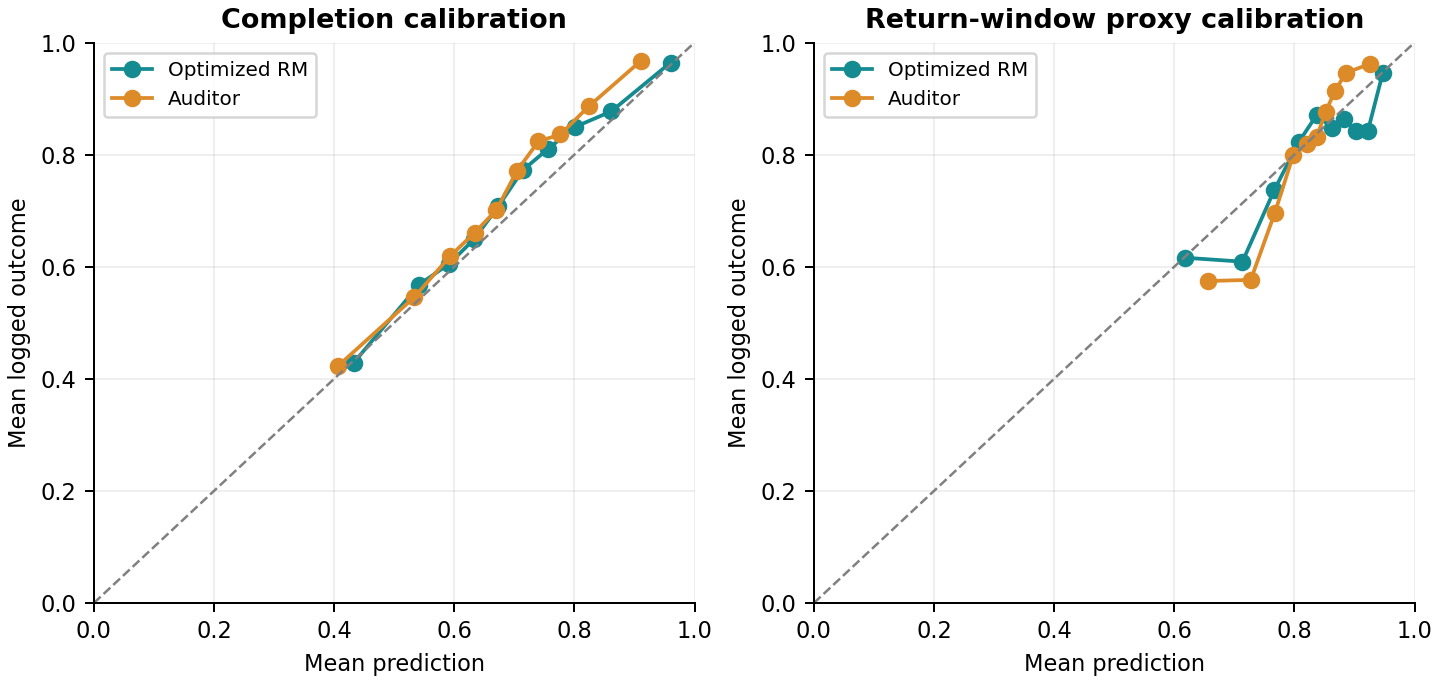
\includegraphics[width=\linewidth,height=.70\textheight,keepaspectratio]{figures/calibration.png}
\caption{Калибровка на реально наблюдавшихся test actions. Она не устанавливает counterfactual calibration.}
\label{fig:calibration}
\end{figure}
